\chapter{Electric and Chromo-electric Dipole Moment of Quarks}
\label{ch:quark(C)EDM}

After the analysis for leptons, we turn our gaze towards EDMs involving quarks. 
However, since quarks are always confined as hadrons, it is extremely difficult, if not outright impossible, 
to directly probe the EDMs of individual quarks, given the state of current technology and our understanding of QCD.
A quick literature~\cite{PDG2022} review shows that there are indeed no direct experimental observations for the EDMs of all the quarks lighter than the top quark.
We comment on the situation of the top quark in \secref{sec:top-cedm}. 
It is natural, under these circumstances, to shift our attention towards hadron EDMs, and utilize the EDM of hadrons to observe the effect of the EDMs of individual quarks.
The prime candidate in this case would be the neutron EDM (\nedm).

\section{The Neutron}
\subsection{Experimental Overview}
Neutron EDM measurements have been in the experimental realm for quite some time already.
The most recent results are given by PSI~\cite{PSI2020nEDM} in 2020, setting the bound at \(|d_{n}| < \num{1.8e-26} \ecm\).
We can use the same back-of-the-envelope mass-scaling estimate that we did for the leptons to estimate the ``equivalent precision'' bound for {\nedm} from the {\eedm} bound.
Since \(m_{u} \sim m_{e} \) and \(m_{d} \) is barely 10 times greater than \(m_{e} \), 
we can place the estimated {\nedm} value at
 \(\sim \num{e-29} \ecm\).
This places the current {\nedm} bound  3-4 orders of magnitude away.

Even though the {\nedm} experimental precision is not as good as that of the {\eedm} experiments,
just looking at the numbers does invoke a \emph{mild} sense of optimism,
especially since this is a \emph{very} naive estimate,
as the dynamics involved in the neutron is much more complicated.
One can reasonably expect the value to be suitably larger.
Unfortunately, that optimistic feeling is quickly extinguished when we take a look at the progress over the past years.
We cite here \figref{fig:snowmass}, taken from the Snowmass conference report~\cite{Snowmass2022EDM}, as a good visual description of {\nedm} experimental progress.
% Figure: Snowmass nEDM experimental status
As can be seen from said figure, progress on the {\nedm} front has stagnated for a decade or so,
with the precision plateauing at \(\sim 10^{-26} \ecm\).
However, we see a silver lining in the report: projects to improve the sensitivity, based on ultra-cold-neutron (UCN) methods, are already in the works.
There is a follow-up project at PSI, named n2EDM~\cite{PSI2021n2EDM}, 
which plans to reach a sensitivity of \(\sim \num{e-27} \ecm \) within a decade.
Furthermore, there is a new experiment under construction at the Spallation Neutron Source~\cite{ORNLnEDM} at Oak Ridge National Laboratory (ORNL),
which projects a precision down to \(\num{e-28} \ecm \).
Nevertheless, it is still worth to explore the {\nedm} parameter space, 
which is what we did~\cite{HKT2024eEDMnEDM}.

\subsection{{\gthdm} Calculations}
As mentioned in the theory section, there are additional chromo-EDM and Weinberg term contributions to take into account that arise from the fact that quarks interact via QCD.
To evaluate the combined combination of these contributions to {\nedm}, we use the more recent formula~\cite{Hisano2014nEDM}
\begin{equation}
  d_n = - 0.20\,d_u + 0.78\,d_d + e\,(0.29\,\tilde d_u + 0.59 \tilde d_d) + e\,23\;{\rm MeV}\,C_W
\end{equation}
instead of the widely cited classic review of Pospelov and Ritz~\cite{PospelovRitz2005EDMs}.
We present the {\gthdm}-with-extended-ansatz~\eqnref{eq:ansatz}-applied calculation results for {\nedm} in \figref{fig:nEDM-fixed}.
% Figure: nEDM results
Interestingly, our predictions for {\nedm} are not too far below the current experimental bound.
We see that, even for \(|\rho_{tt}| = 0.3\sqrt{2} \approx 0.42\), one can still survive the current PSI bound.
The projected \(\sim \num{e-27} \ecm \) sensitivity of n2EDM at PSI covers the range illustrated in \figref{fig:nEDM-fixed},
putting stress on our model.
Fortunately, there is still a possibility of lowering the predicted {\nedm} value of our model 
should the new experimental bounds indeed close in.

So far, we have been utilizing the ``extended'' cancellation ansatz~\eqnref{eq:ansatz} in our above calculations and analyses.
However, we have to reiterate that it is merely a convenient way to numerically illustrate the \textit{flavor hierarchy} of the {\gthdm}.
A closer examination of the ``extended'' ansatz reveals a logical flaw: 
since \(\rho_{uu} \) and \(\rho_{tt} \) are in the same \(\rho \) matrix, and the ansatz obviously does not hold for \(\rho_{tt} \) itself, 
there is no reason to expect it to hold for \(\rho_{uu} \).
Thus, for this situation, we should fall back one step, and rely on the \textit{rule of thumb}~\eqnref{eq:ruleofthumb} instead of the ansatz.
Hence, we relax the ansatz for \(\rho_{uu} \), and explore the range of \(\order{\lambda_{u}} \) by varying
\begin{equation}
  |\rho_{uu}| \in [0.3\lambda_u, 3\lambda_u], \quad \arg\rho_{uu} \in [-\pi, \pi]
\end{equation}
while keeping the other \(\rho_{ff} \)s intact, i.e. still following the ansatz.
We present our results for said variation in \figref{fig:nEDM-varied}.
% Figure: nEDM varying rho_uu
The different colors of the points represent different values of \(\arg\rho_{uu} \), and an interesting pattern can be seen among them.
The red points have negative \(\arg\rho_{uu} \), which is the same sign as \(\rho_{tt} \); 
the {\nedm} of these points are larger, but stay mostly below the PSI bound.
On the other hand, the blue points have \textit{positive} \(\arg\rho_{uu} \), which is the \textit{opposite} sign as \(\rho_{tt} \); 
remarkably, the value of {\nedm} of these points drop significantly, reaching as low as \(\num{e-28} \ecm \) or lower, 
evading even the projected sensitivity of n2EDM!
This phenomenon in \figref{fig:nEDM-varied} illustrates a \textit{natural} cancellation mechanism present within the dynamics of {\nedm},
arising from the phase difference of \(\rho_{uu} \) and the other \(\rho_{ff} \).
Even though this mechanism can evade the projected n2EDM sensitivity, 
it can still be probed by the SNS at ORNL, with its down to \(\sim \num{e-28} \ecm \) projected sensitivity.
This experiment may take more than a decade to come to fruition, but it almost fully covers our projected range, since the blue dots are still mostly concentrated above \(\num{e-28} \ecm \).

\clearpage
% Snowmass nEDM experimental status
\begin{figure}[p]
    \centering
    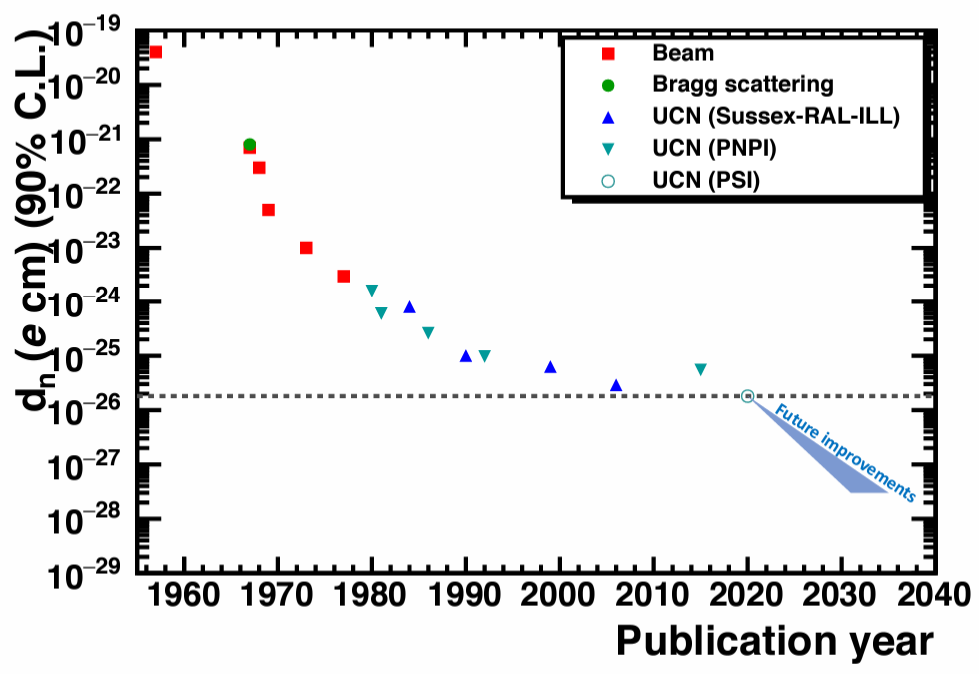
\includegraphics[width=0.5\linewidth]{Snowmass_fig.png}
    \caption{nEDM experimental progress~\cite{Snow22}}
    \label{fig:snowmass}
\end{figure}

% nEDM fixed rho_uu
\begin{figure}[p]
    \centering
    \begin{minipage}{0.48\textwidth}
      \centering
      \includegraphics[width=0.85\linewidth]{example-image}
      \caption{nEDM results.}
      \label{fig:nEDM-fixed}
    \end{minipage}\hfill
    \begin{minipage}{0.48\textwidth}
      \centering
      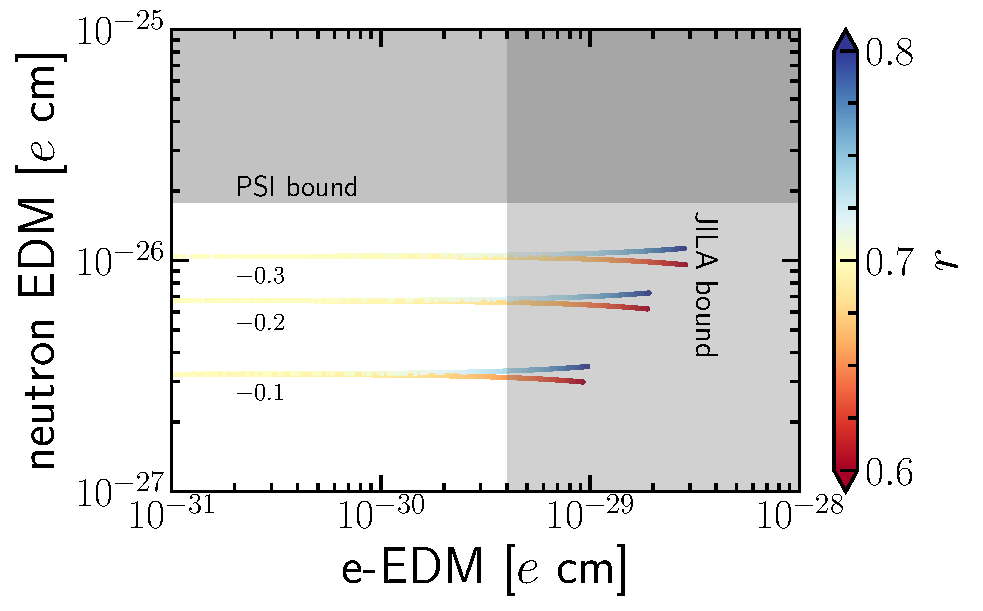
\includegraphics[width=0.95\linewidth]{fig3.pdf}
      \caption{Combined eEDM-nEDM result.}
      \label{fig:nEDM-eEDM}
    \end{minipage}
\end{figure}

% nEDM varying rho_uu
\begin{figure}[p]
    \centering
    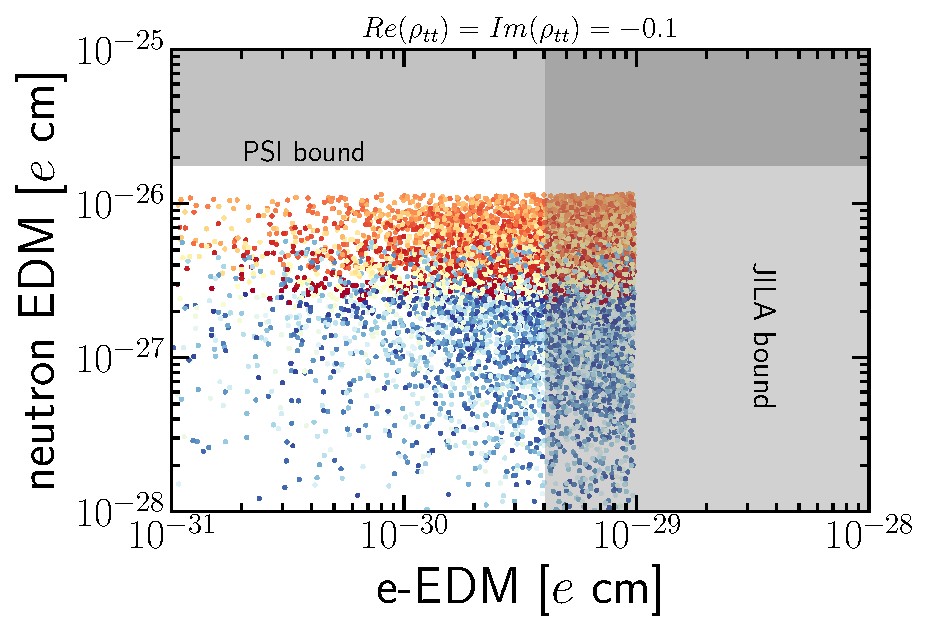
\includegraphics[width=7.35cm,height=5.55cm,angle=-90]{fig4_1.pdf}\\
    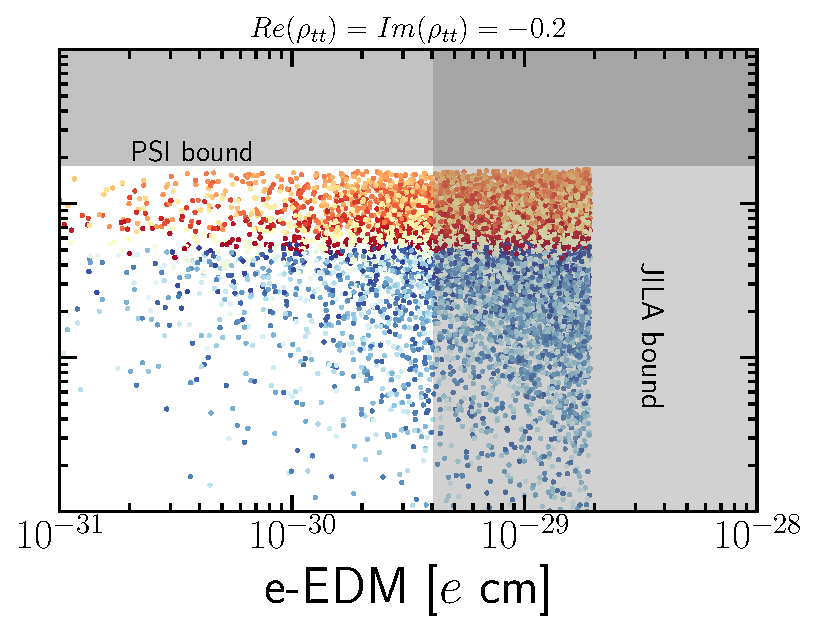
\includegraphics[width=6.45cm,height=5.55cm,angle=-90]{fig4_2.pdf}\\
    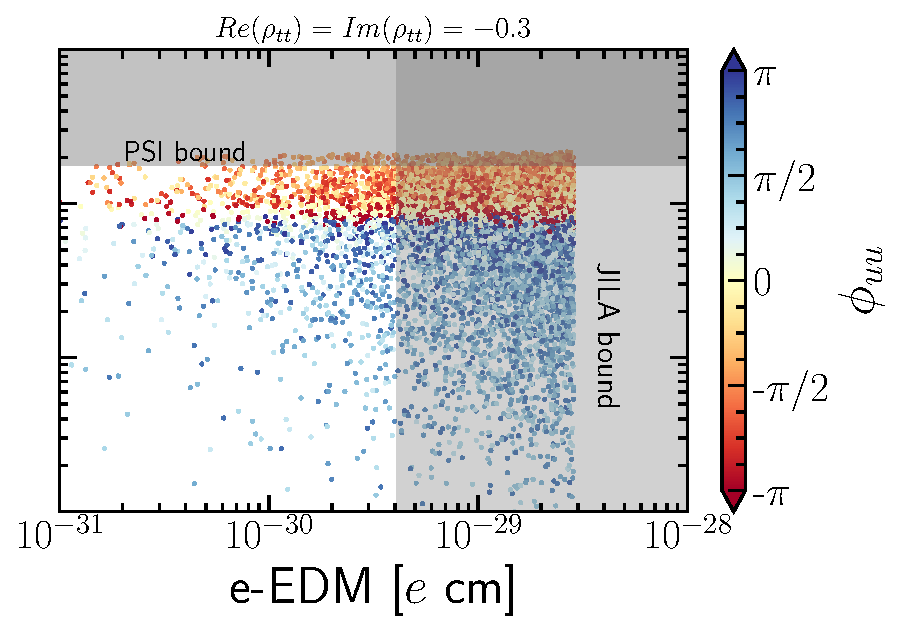
\includegraphics[width=7.89cm,height=5.55cm,angle=-90]{fig4_3.pdf}
    \caption{Results for eEDM and nEDM with \(|\rho_{uu}| \sim \lambda_{u}\).}
    \label{fig:nEDM-varied}
\end{figure}